\subsection{问题三：算力约束下的资源配置与结构性转移}
\begingroup
\setlength{\tabcolsep}{5pt}

\subsubsection{问题分析与模型准备}

我们在同一训练预算下联合配置参数量、数据量与质量。扩大参数规模会降低参数项损失，同时提高每个 token 的训练费用；改善质量会缩小质量缺口，同时增加整份语料的处理成本。两项投入都会挤占数据训练预算，因此配置时需要比较直接收益与数据量减少带来的损失。

已有研究给出了固定算力下参数和数据的配置关系\cite{hoffmann2022chinchilla}。考虑到题设还包含质量处理与长上下文计算，我们以问题二的损失函数为目标，加入相应费用约束，先求不同预算下的配置，再检验结论对成本形式的依赖。

图\ref{fig:p3_workflow}梳理了本问的计算过程。先汇入前两问的质量基线、配比修正与损失参数，再将训练、质量处理和注意力费用写入预算约束。多初值求解后，分别比较三档预算配置、连续预算中的质量投入阶段，以及成本形式和上下文改变时的配置差异。

\begin{figure}[!htbp]
 \centering
 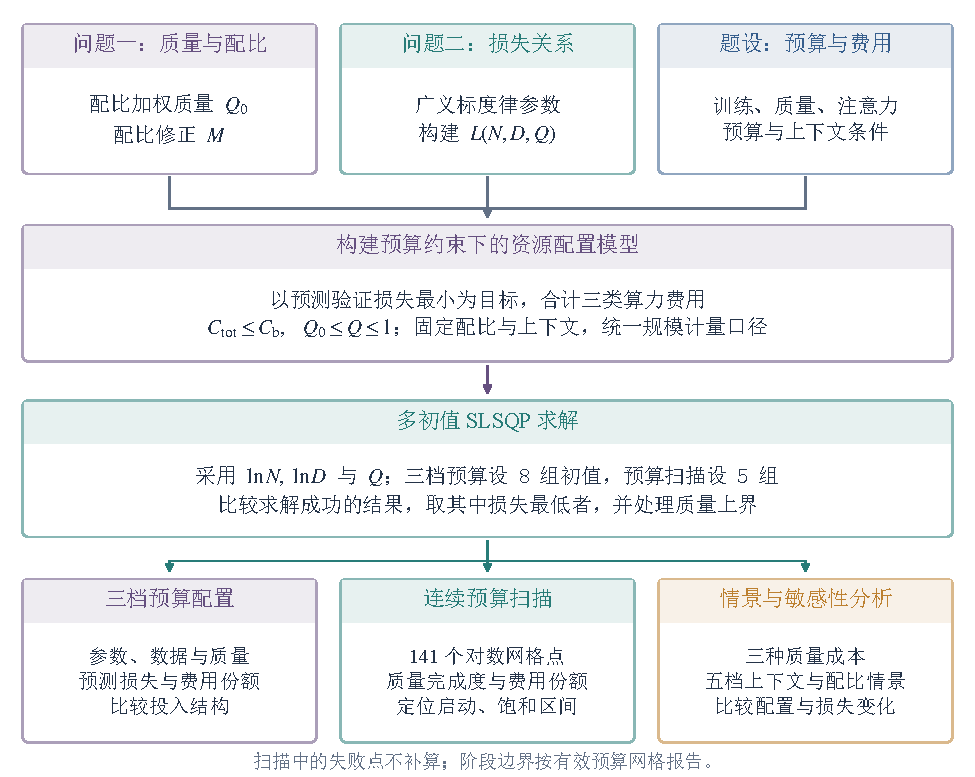
\includegraphics[width=0.94\textwidth]{figures/q3-workflow.pdf}
 \caption{问题三资源配置与求解流程}
 \label{fig:p3_workflow}
\end{figure}

\par\medskip\noindent\textbf{数据与计算口径}\par

本问直接使用问题二估计的损失参数。其中规模项为 $A=0.3808$、$\alpha=0.3266$、$B=1.2515$、$\beta=0.2767$，质量项为 $C_q=0.3544$、$\gamma=0.9779$，常数项为 $E=1.6558$。质量系数改记 $C_q$，以区别预算 $C_{\mathrm b}$。计算费用时，$N$、$D$ 分别用参数个数与 token 个数；代入损失式时再换成 $n=N/10^9$、$d=D/10^9$。下列表格的 B 均表示十亿。

求解器以绝对数量的对数为变量，计算目标和约束时还原规模，再分别用于损失与费用计算。后文的一阶条件也先换算系数，再对绝对数量求导，保持两种计量口径一致。

我们先以参考配方确定质量处理的起点。用 A4 的平均配比 $\bar p_k$ 加权问题一经 A16 映射的领域评分 $Q_k$，得到基线
\[
 Q_0=\sum_{k=1}^{17}\bar p_kQ_k=0.5487.
\]
这里沿用 A4 原始平均份额得到外生成本基线 $Q_0=0.548688$。问题一求核岭配比时将参考份额归一化至和为 1，其加权质量为 0.548753；两种口径分别记录，不因配比归一化而重设本问的费用起点。全量文本均值 $0.4912$ 另作灵敏度对照。

记问题一评分为 $Q_A$、附件 B 评分为 $Q_B$，本问采用 $Q_B=h(Q_A)=Q_A$，并在共同数值轴上计算费用。恒等映射是缺少配对标定资料时的情景假设。优化范围为 $Q_0\le Q\le1$，满分只表示模型质量上界。

配比比较保持共同 $Q_0$，只对超过该基线的质量计费。核岭候选自身的加权质量为 0.5182，换配方后原料质量并不相同。若按各配方质量 $Q_0(\bm p)$ 分别计费，就需要另行求解配比与处理成本的耦合；本节先单独比较固定损失平移，随后给出更换费用基线的对照。

基准情景取参考配比 $M=0$、幂函数成本及 $2048$ tokens 上下文；成本类型和上下文依次改变。附件 C7 的 2048、4096、8192、32768、131072 tokens 均作为给定条件，求解器只调整参数、数据与质量。此外，将核岭配比对应的 $M=-0.1730$ 单列为收益情景，检查损失与等效预算如何变化。

\subsubsection{模型建立}

\textbf{1.每个训练 token 的算力代价}\par\nopagebreak[4]
基础训练使用 $6ND$ 的成本近似\cite{hoffmann2022chinchilla}，质量与注意力费用按照题目第三问及题目附录 B 的成本设定计算。由于三类 $g(Q)$ 在允许范围内均递增，可记质量提升的单位增量费用为 $\Delta g(Q)=g(Q)-g(Q_0)\ge0$，从而将总成本写为
\begin{equation}
 C_{\mathrm{tot}}
 =6ND+D\Delta g(Q)+\eta ND L_{\mathrm{ctx}}
 =D\underbrace{\left[(6+\eta L_{\mathrm{ctx}})N+\Delta g(Q)\right]}_{\text{单位 token 的合计算力成本}},
 \qquad \eta=2\times10^{-4}.
 \label{eq:p3_cost_total}
\end{equation}
三项费用都随数据量 $D$ 累计。给定 $N,Q$ 时，每个新增 token 的单价不变；提高质量则增加整份语料的处理费用，压缩可用于训练的数据量。即使质量已达上界，新增数据仍需支付处理费用。

这里的 $D$ 按累计训练 token 数使用，质量费用也按相同数量核算，尚未扣除重复使用语料可能带来的处理成本复用。若一份语料仅预处理一次、随后多轮训练，应区分独立语料量与累计训练量；当前算例沿用题设费用，不对这类复用作额外修正。

表\ref{tab:p3_functions}列出题设的三种质量成本。由于比较的是相对基线的增量 $\Delta g(Q)$，三种函数在 $Q_0$ 处均不产生额外费用。
\begin{table}[htbp]
 \centering
 \normalfont\normalsize\color{black}
 \renewcommand{\arraystretch}{1.15}
 \caption{质量处理成本函数（$g$ 的单位为 FLOPs/token）}
 \label{tab:p3_functions}
 \begin{tabularx}{0.98\textwidth}{@{}*{3}{>{\centering\arraybackslash}X}@{}}
 \toprule
 成本类型 & $g(Q)$ & 本节用途\\
 \midrule
 幂函数型 & $5\times10^9Q^4$ & 基准配置\\
 指数型 & $10^7e^{6Q}$ & 成本形式对照\\
 对数渐进型 & $2\times10^9\ln(1+10Q)$ & 成本形式对照\\
 \bottomrule
 \end{tabularx}
\end{table}

\textbf{2.预算约束下的配置模型}\par\nopagebreak[4]
记 $k=6+\eta L_{\mathrm{ctx}}$。给定配比和上下文长度后，以预测验证损失最小为目标，得到
\begin{equation}
 \begin{aligned}
 \min_{N,D,Q}\quad &E+A n^{-\alpha}+B d^{-\beta}+C_q(1-Q)^\gamma+M,\\
 \mathrm{s.t.}\quad&D\,[kN+\Delta g(Q)]\le C_{\mathrm b},\qquad Q_0\le Q\le1,\\
 &10^5\le N\le10^{15},\qquad 10^6\le D\le10^{16}.
 \end{aligned}
 \label{eq:p3_problem}
\end{equation}
末尾界限限定数值搜索范围，不代表实际数据供给。共同 $Q_0$ 固定、配比可行域独立且 $M(\bm p)$ 可加分离时，先最小化 $M$ 再优化 $N,D,Q$，与联合最小化等价；若基线或费用随配比变化，这种分离便不再成立。本文使用问题一多初值求得的核岭候选，不据此保证全局最优或真实训练收益。因此，“配比改变而配置不变”来自模型设定。

固定质量且规模界限不活跃时，增加 $N$ 或 $D$ 都能降低损失，预算约束因而取等号。将其写为
\begin{equation}
 D=\frac{C_{\mathrm b}}{kN+\Delta g(Q)}
 \label{eq:p3_budget_balance}
\end{equation}
预算式说明，提高 $N$ 或 $Q$ 后，能够负担的 $D$ 都会减少。因此，我们比较一项投入的净收益时，同时计入其直接降低的损失与数据缩减增加的损失。

预算用尽可由数据项的单调性说明：在 $N,Q$ 固定、数据上界未达到时，增加 $D$ 只会减小 $Bd^{-\beta}$。若仍有余款，就还可降低损失。消去数据量后，可在预算边界上比较参数与质量；以下用该化简解释一阶条件，正式程序仍求解三变量约束模型。

由式\eqref{eq:p3_budget_balance}还可分别求得预算固定时的数据变化：
\begin{equation}
 \left.\frac{\partial D}{\partial N}\right|_Q
 =-\frac{kD}{kN+\Delta g(Q)},\qquad
 \left.\frac{\partial D}{\partial Q}\right|_N
 =-\frac{Dg'(Q)}{kN+\Delta g(Q)}.
 \label{q3_expand_data_tradeoff}
\end{equation}
两项均为负，分别对应扩大模型和提高质量带来的数据缩减。质量成本的影响还取决于当前位置的斜率 $g'(Q)$，因而不能只比较不同成本函数在某一个质量水平上的取值。这也说明，费用形式相近的情景仍可能产生不同的质量选择。

\textbf{3.参数量与数据量的平衡}\par\nopagebreak[4]
为统一求导单位，先令 $\widetilde A=A(10^9)^\alpha$、$\widetilde B=B(10^9)^\beta$，把规模项改写为绝对数量形式。固定 $Q$ 后，将预算等式\eqref{eq:p3_budget_balance}代入损失函数，可得
\[
 F(N)=\widetilde A N^{-\alpha}
      +\widetilde B\left[\frac{kN+\Delta g(Q)}{C_{\mathrm b}}\right]^\beta.
\]
此处省略的常数项和质量项在固定质量后不随 $N$ 变化，不影响导数。参数项的导数为负，数据项则因预算挤占而产生正导数，两者相加为
\begin{equation}
 F'(N)=-\alpha\widetilde A N^{-\alpha-1}
 +\frac{\beta\widetilde Bk}{C_{\mathrm b}^{\beta}}
       [kN+\Delta g(Q)]^{\beta-1}.
 \label{q3_expand_parameter_derivative}
\end{equation}
令该式为零，再乘以 $[kN+\Delta g(Q)]/k$，并用预算等式替换数据项，即可得到参数与数据损失的平衡关系。
对应的平衡式为
\begin{equation}
 \alpha\widetilde A N^{-\alpha}
 \left(1+\frac{\tau(Q)}{N}\right)
 =\beta\widetilde B D^{-\beta},
 \qquad \tau(Q)=\frac{\Delta g(Q)}k.
 \label{eq:p3_balance}
\end{equation}
为解释式\eqref{eq:p3_balance}，可把 $\tau(Q)$ 看作质量费用折算出的附加参数规模，它与 $N$ 单位相同。因而，因子 $1+\tau/N$ 表示额外质量处理对规模平衡的影响。一旦为质量付费，原本只在参数与数据之间分配的方案就需要随之调整。

作为对照，保持基线质量时有 $\tau=0$，于是 $\alpha\widetilde A N^{-\alpha}=\beta\widetilde B D^{-\beta}$。将其与 $kND=C_{\mathrm b}$ 联立，在上下文固定时得到
\begin{equation}
 N^*\propto C_{\mathrm b}^{\beta/(\alpha+\beta)},\qquad
 D^*\propto C_{\mathrm b}^{\alpha/(\alpha+\beta)}.
 \label{eq:p3_scaling}
\end{equation}
不额外提高质量时，数据量随预算增长稍快于参数量：两者的指数分别约为 $0.541$、$0.459$。这只是基线质量下的参照；开始投入质量后，应回到包含处理费用的完整模型计算。

基线幂律的比例系数也可由同一组方程求出。将 $D=C_{\mathrm b}/(kN)$ 代入平衡条件，得到
\begin{equation}
 \begin{aligned}
 (N^*)^{\alpha+\beta}
 &=\frac{\alpha\widetilde A}{\beta\widetilde B}
   \left(\frac{C_{\mathrm b}}{k}\right)^\beta,\\
 N^*&=\left(\frac{\alpha\widetilde A}{\beta\widetilde B}\right)^{1/(\alpha+\beta)}
       \left(\frac{C_{\mathrm b}}{k}\right)^{\beta/(\alpha+\beta)},\\
 D^*&=\left(\frac{\beta\widetilde B}{\alpha\widetilde A}\right)^{1/(\alpha+\beta)}
       \left(\frac{C_{\mathrm b}}{k}\right)^{\alpha/(\alpha+\beta)}.
 \end{aligned}
 \label{q3_expand_baseline_closed_form}
\end{equation}
因此，预算通过幂指数决定规模的增长速度，系数比值决定具体配置水平。上下文固定时，$k$ 只进入有效预算因子；质量费用不为零时，预算中多出无法并入 $kN$ 的处理项，基线表达式便不再适用于完整配置。因此，该解析式只适用于没有质量增量费用的参照情形，用来解释规模权衡；完整配置仍由含质量费用的预算模型求解。

质量选择也可在同一预算边界上解释。当预算约束活跃、数据量未触及搜索上下界且 $Q_0<Q<1$ 时，固定 $N$ 并对消去数据量后的损失求导，质量最优的必要条件为
\begin{equation}
 \frac{\beta\widetilde B D^{-\beta}g'(Q)}{kN+\Delta g(Q)}
 =\gamma C_q(1-Q)^{\gamma-1}.
 \label{q3_expand_quality_balance}
\end{equation}
式中左侧是质量提升挤占数据预算后增加的损失，右侧是质量改善直接减少的损失。我们据此将内部配置解释为两项边际作用相抵的结果。若解位于基线或质量上界，应结合允许的变化方向判断，不能要求上述等式成立。尤其在上界处，质量项的导数性质与内部不同。因此，本问的阶段位置仍依据后文的预算扫描确定，一阶条件用于解释内部配置的局部权衡。

\textbf{评分尺度的条件对照。} 为检查恒等映射的影响，我们保留 $Q_A$ 轴上的幂函数费用，分别令 $Q_B=h(Q_A)$ 取 $\sqrt{Q_A}$、$Q_A$、$Q_A^2$。三者方向及端点相同，但固定 $N,D$ 时，质量项关于处理评分的损失导数变为
\begin{equation}
 -\frac{\partial L}{\partial Q_A}
 =C_q\gamma[1-h(Q_A)]^{\gamma-1}h'(Q_A).
 \label{eq:q23_review_quality_mapping}
\end{equation}
在参考配比、2048 tokens 上下文及基线规模最优曲线上，以质量收益与预算挤占损失的一阶平衡确定下界释放点，得到表\ref{tab:q23_review_quality_scale}。该点说明何时从基线小幅提高质量开始有利，存在竞争端点时不一定等于全局阶段边界。

\begin{table}[htbp]
 \centering
 \caption{评分映射改变时的局部质量投入释放点}
 \label{tab:q23_review_quality_scale}
 \renewcommand{\arraystretch}{1.15}
 \begin{tabularx}{0.94\textwidth}{@{}*{3}{>{\centering\arraybackslash}X}@{}}
 \toprule
 映射 $h(Q_A)$ & 参考基线在 B 轴的值 & 释放预算（$10^{19}$ FLOPs） \\
 \midrule
 $\sqrt{Q_A}$ & 0.7407 & 2.94 \\
 $Q_A$ & 0.5487 & 1.57 \\
 $Q_A^2$ & 0.3011 & 1.37 \\
 \bottomrule
 \end{tabularx}
\end{table}

这些映射用于检验同向评分并不唯一决定投入阈值，没有被当作新的标定结果。基准情景仍用恒等映射；其他处理评分或实际费用若定义在不同尺度上，应先同步转换损失与费用，再使用相应配置。

\textbf{4.数值求解与阶段识别}\par\nopagebreak[4]
我们采用 SciPy 的 SLSQP 实现\cite{scipy_slsqp}求解式\eqref{eq:p3_problem}，以 $\ln N$、$\ln D$ 缩小变量尺度差异，并将预算不等式等价写为 $1-C_{\rm total}/C_{\mathrm b}\ge0$，避免约束绝对量级过大；停止条件取 ftol=$10^{-14}$，单次求解最多迭代 1500 次。三档预算各设 8 组初值，连续预算扫描各设 5 组，从求解成功的结果中选取损失最低的一组，记作 $(N^*,D^*,Q^*)$。这样可降低初值和局部解的影响，但不能保证全局最优。另因 $\gamma<1$ 时 $Q=1$ 的导数无界，将达到该上界的配置作为边界解处理。将保存的配置重新代入成本函数，三档预算、上下文敏感性与全部 141 个预算扫描点的最大相对预算残差均小于 $10^{-12}$。这些数值核验说明记录的配置满足预算约束，但只验证可行性，不构成对全局最优性的证明。

对数变量使参数量与数据量的正值约束自然满足，原有规模上下界相应转换为对数区间。实际初值设置让参数量与数据量沿相反方向变化，同时使质量起点分布在允许区间内部，以比较不同资源组合出发后的求解结果。每次求解都保留总预算不等式和质量边界，而不是先独立确定三项投入后再缩放预算。成功状态用于筛选候选结果，边界配置则保留其实际质量值；未记录成功结果的预算点不参与后续阶段定位。多初值比较用于同一预算下的候选选择，相邻预算点仍分别求解，阶段变化依据有效输出识别。

质量投入的阶段用完成度 $\Theta=(Q^*-Q_0)/(1-Q_0)$ 表示，质量处理占预算的份额用 $f_Q=D^*\Delta g(Q^*)/C_{\mathrm b}$ 表示。完成度为 0 时维持基线，介于 0、1 时正在提升，等于 1 时达到上界。计算在 $10^{18}$--$10^{25}$ FLOPs 内设置 141 个对数等距点，相邻预算之比约为 1.122，逐点寻找首次投入与首次饱和的位置。采用无量纲预算约束后，141 个网格点均取得有效配置，阶段分析使用全部输出。

我们同时观察完成度与费用份额，以区分质量提升的进度和资源支出。前者以可提升的质量区间为分母，后者以总预算为分母；质量不变时，规模调整仍可能改变费用份额。因此，质量曲线变平不表示处理费用消失，阶段位置也只能由有效预算网格点定位。

\subsubsection{模型求解}

图中坐标、费用份额及网格判定的计算口径见附录 F。

\noindent\textbf{辅助分析说明：} 本问的文段相关辅助参考腾讯 WorkBuddy 接入的 DeepSeek-V4-Flash（2026-07-31 公开测试），图表展示、程序整理与复现核对使用 OpenAI Codex（GPT-5.6-Luna，2026-07-09）\cite{ai_workbuddy,ai_deepseek,ai_codex56luna}。正文表达与段落衔接另经 OpenAI Codex 辅助润色。

\textbf{1.预算增加后，质量与规模如何分配}\par\nopagebreak[4]
比较表\ref{tab:p3_opt}中的三档配置，我们发现各项投入并未按相同比例增长。参数和数据都在增加，但数据更快，$D/N$ 由 30.9 升到 76.1。质量在低预算档停留于基线，中、高预算档则达到上界，不能简单地按固定比例同时扩张三项投入。

\begin{table}[htbp]
 \centering
 \normalfont\normalsize\color{black}
 \renewcommand{\arraystretch}{1.15}
 \caption{三档预算的基准配置（幂函数型成本，$L_{\mathrm{ctx}}=2048$，$M=0$）}
 \label{tab:p3_opt}
 \begin{tabularx}{0.98\textwidth}{@{}*{7}{>{\centering\arraybackslash}X}@{}}
 \toprule
 \makecell{预算\\（FLOPs）} & $N^*$（B） & \makecell{$D^*$\\（B tokens）} & $Q^*$ & $L^*$ & $D^*/N^*$ & $f_Q$（\%）\\
 \midrule
 $10^{19}$ & 0.225 & 6.9 & 0.549 & 3.171 & 30.9 & 0.0 \\
 $10^{22}$ & 6.091 & 229.4 & 1.000 & 2.145 & 37.7 & 10.4 \\
 $10^{24}$ & 44.939 & 3417.8 & 1.000 & 1.897 & 76.1 & 1.6 \\
\bottomrule
 \end{tabularx}
\end{table}

为定位质量投入的阶段变化，我们继续沿用幂函数型成本、$L_{\mathrm{ctx}}=2048$、$M=0$ 作预算扫描。图\ref{fig:p3_shift}左侧为完成度，右侧为三类费用份额，内嵌小图放大了质量提升区间。两条竖线对应首次启动和首次饱和的有效网格点；曲线连接逐点求解得到的记录。
\begin{figure}[htbp]
 \centering
 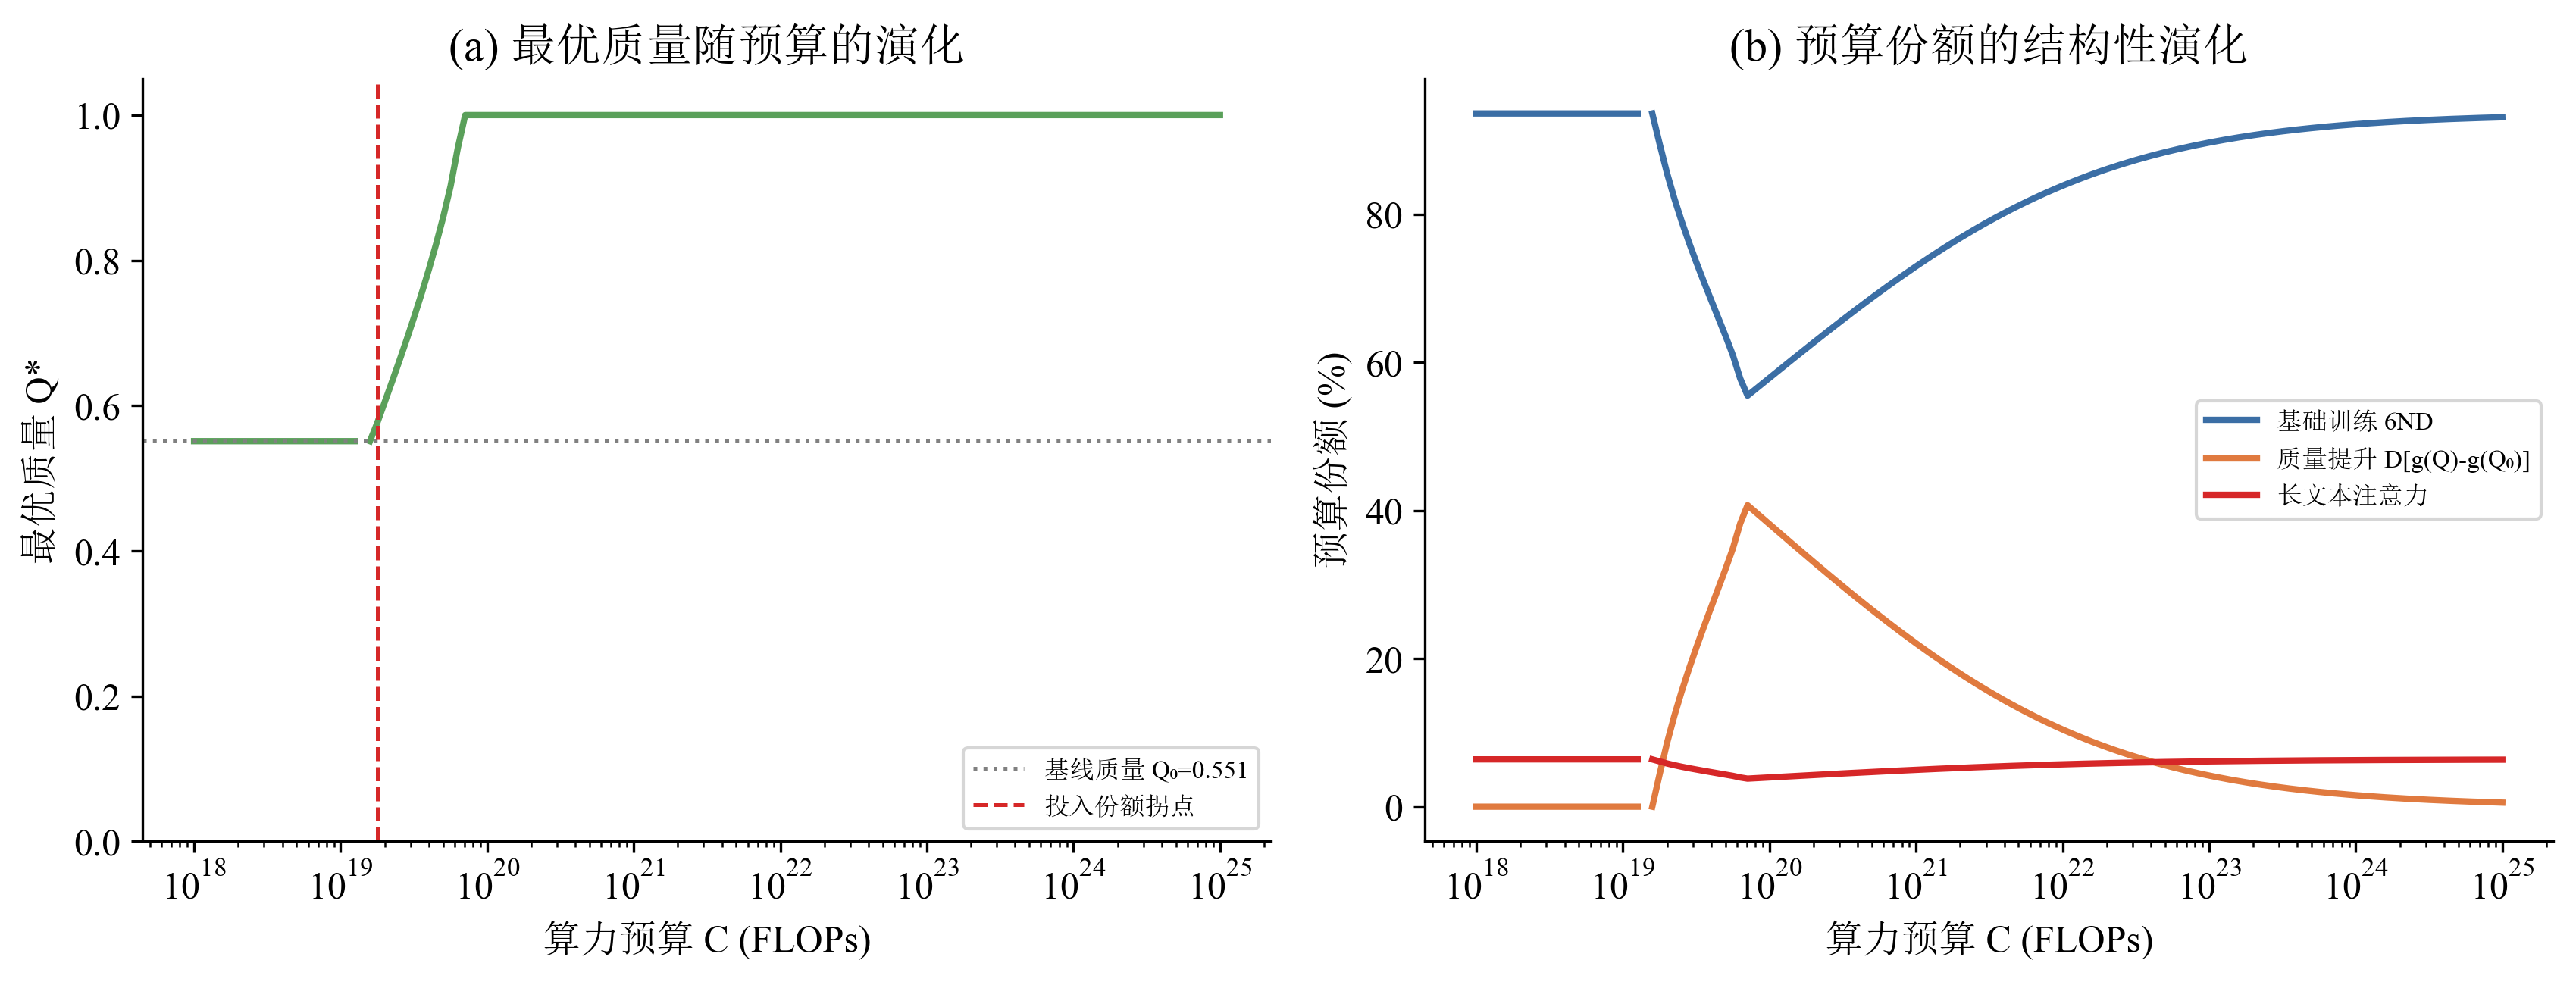
\includegraphics[width=0.94\textwidth]{../求解/问题三/图片/图2_预算份额结构性转移.png}
 \caption{给定标度律参数下的预算与费用份额}
 \label{fig:p3_shift}
\end{figure}

低预算的有效解都保持 $Q^*=Q_0$。此时 $93.6\%$ 用于基础训练，$6.4\%$ 用于注意力计算。虽然提高质量可降低质量项损失，但它会占用原本可用于数据训练的费用；在当前成本设定下，数值比较选择维持基线。

费用份额的变化可进一步从预算等式得到解释。记基础训练和注意力的份额分别为 $f_{\mathrm{train}}$、$f_{\mathrm{attn}}$，预算充分使用时有
\begin{equation}
 f_{\mathrm{train}}=\frac{6N^*}{kN^*+\Delta g(Q^*)},\qquad
 f_{\mathrm{attn}}=\frac{\eta L_{\mathrm{ctx}}N^*}{kN^*+\Delta g(Q^*)},\qquad
 f_{\mathrm{train}}+f_{\mathrm{attn}}+f_Q=1.
 \label{q3_expand_budget_shares}
\end{equation}
上下文固定时，基础训练与注意力的费用比保持不变。质量投入出现后，这两项在总预算中的份额会共同受到压缩，但彼此的比例仍由上下文决定。因此，图中的三类份额并非能够任意调整的三个独立变量，其变化受到成本结构的约束。

质量投入的两个变化位置可以从扫描点看出。到 $1.58\times10^{19}$ FLOPs，首次出现额外质量费用；到 $7.08\times10^{19}$ FLOPs，质量达到上界，费用份额也升至峰值 $40.7\%$。在后一位置之前，最近有效点的质量约为 0.956。结合相邻点，启动区间为 $[1.41,1.58]\times10^{19}$ FLOPs，饱和区间为 $[6.31,7.08]\times10^{19}$ FLOPs。这些是当前网格的定位范围，精确临界值并未由扫描确定。

上述区间仅反映原参数和当前网格。表\ref{tab:q23_review_gamma}中，$\gamma=1$ 的受限拟合与原拟合目标接近，却使原首次饱和点的质量变为 0.9640，说明网格定位误差之外还存在函数形状的不确定性。因此，三阶段图用于解释现有情景，不将两个网格区间当作已经验证稳健的投入门槛。

达到质量上界后，$Q$ 已不能继续增加，新增预算主要用于扩参数和数据。此时单位质量费用固定为 $\Delta g(1)$，预算关系给出
\[
 f_Q=\frac{\Delta g(1)}{kN^*+\Delta g(1)}.
\]
达到上界后，模型越大，质量费用份额越小，至 $10^{24}$ FLOPs 约为 $1.6\%$。这是训练费用增长更快造成的，不能理解为质量处理总支出减少，因为每个新增 token 仍承担同样的处理费用。质量不再增加也来自上界约束，而非边际收益归零；问题二估计的 $\gamma$ 仍小于 1。

\FloatBarrier

\textbf{2.低预算的质量选择取决于成本形式}\par\nopagebreak[4]
我们进一步更换质量成本形式，检查上述阶段是否依赖幂函数设定。保持 $L_{\mathrm{ctx}}=2048$、$M=0$，用表\ref{tab:p3_functions}的三种函数分别求解。图\ref{fig:p3_cost}对照九组结果的质量及费用份额，表\ref{tab:p3_cost}列出对应规模配置。
\begin{figure}[htbp]
 \centering
 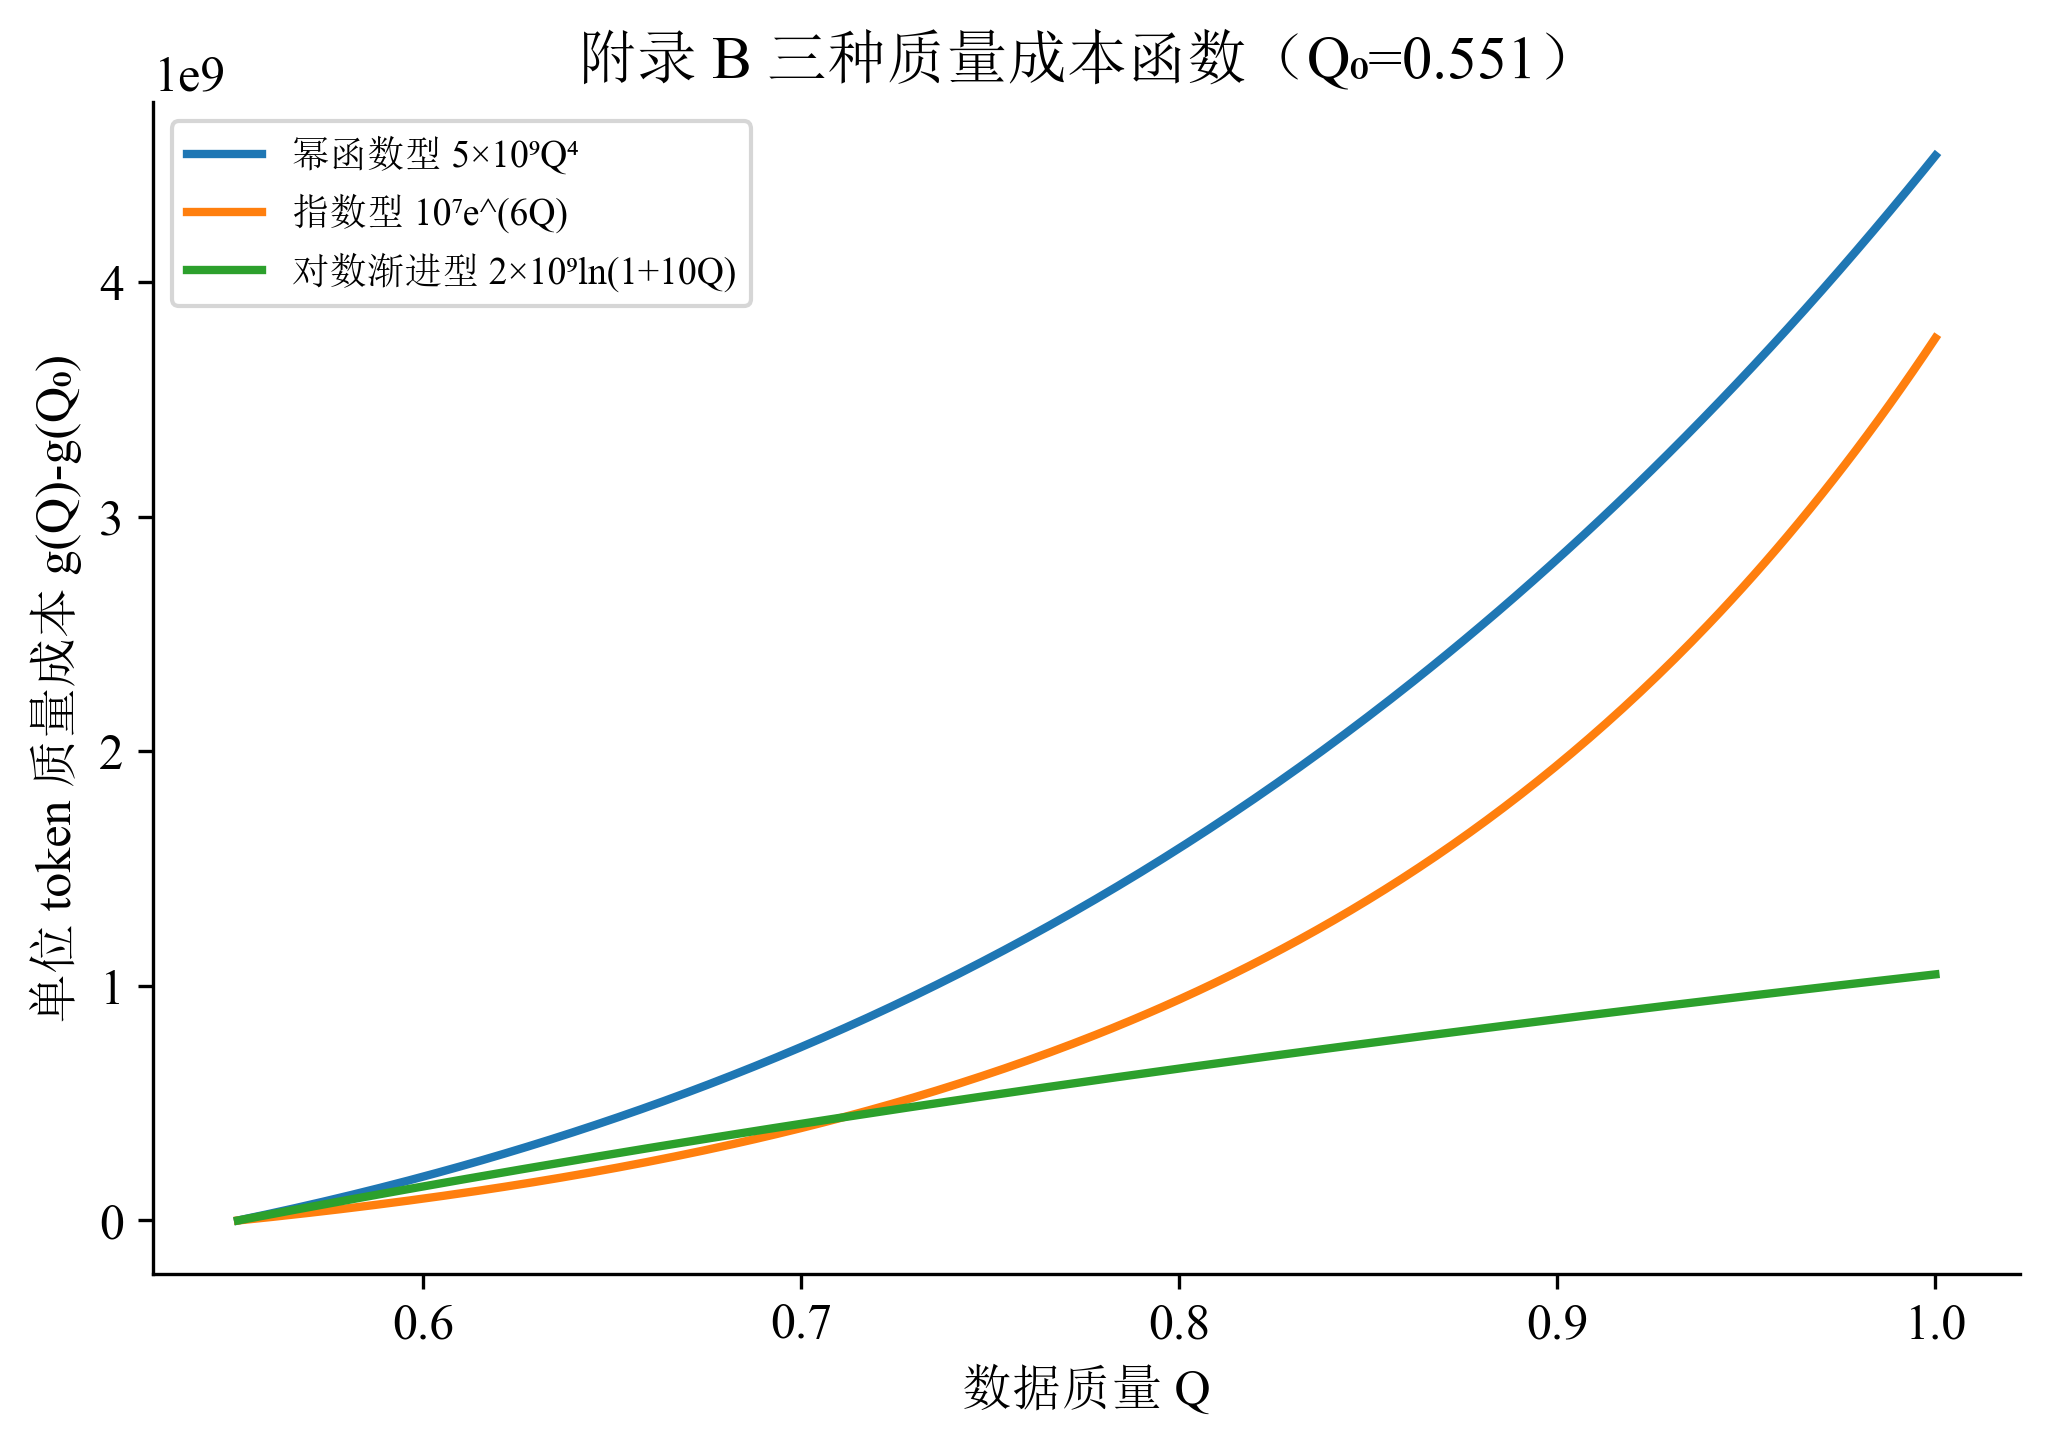
\includegraphics[width=0.94\textwidth]{../求解/问题三/图片/图4_质量成本函数对比.png}
 \caption{成本函数比较}
 \label{fig:p3_cost}
\end{figure}

\begin{table}[htbp]
 \centering
 \normalfont\normalsize\color{black}
 \renewcommand{\arraystretch}{1.15}
 \caption{三类质量成本下的配置对比（$L_{\mathrm{ctx}}=2048$，$M=0$）}
 \label{tab:p3_cost}
 \begin{tabularx}{0.98\textwidth}{@{}>{\hsize=0.95\hsize\linewidth=\hsize\centering\arraybackslash}X>{\hsize=1.4\hsize\linewidth=\hsize\centering\arraybackslash}X>{\hsize=0.93\hsize\linewidth=\hsize\centering\arraybackslash}X>{\hsize=0.93\hsize\linewidth=\hsize\centering\arraybackslash}X>{\hsize=0.93\hsize\linewidth=\hsize\centering\arraybackslash}X>{\hsize=0.93\hsize\linewidth=\hsize\centering\arraybackslash}X>{\hsize=0.93\hsize\linewidth=\hsize\centering\arraybackslash}X@{}}
 \toprule
 \makecell{预算\\（FLOPs）} & 成本类型 & $N^*$（B） & \makecell{$D^*$\\（B tokens）} & $Q^*$ & $L^*$ & $f_Q$（\%）\\
 \midrule
 $10^{19}$ & 指数型 & 0.266 & 5.1 & 0.660 & 3.163 & 13.1 \\
  & 幂函数型 & 0.225 & 6.9 & 0.549 & 3.171 & 0.0 \\
  & 对数渐进型 & 0.355 & 3.0 & 1.000 & 3.113 & 31.7 \\
 \addlinespace[4pt]
 $10^{22}$ & 指数型 & 5.972 & 237.8 & 1.000 & 2.144 & 9.0 \\
  & 幂函数型 & 6.091 & 229.4 & 1.000 & 2.145 & 10.4 \\
  & 对数渐进型 & 5.528 & 274.1 & 1.000 & 2.139 & 2.9 \\
 \addlinespace[4pt]
 $10^{24}$ & 指数型 & 44.797 & 3437.6 & 1.000 & 1.897 & 1.3 \\
  & 幂函数型 & 44.939 & 3417.8 & 1.000 & 1.897 & 1.6 \\
  & 对数渐进型 & 44.300 & 3508.8 & 1.000 & 1.897 & 0.4 \\
\bottomrule
 \end{tabularx}
\end{table}

在 $10^{19}$ FLOPs 时，幂函数成本得到的质量是 0.549，指数型为 0.660，对数渐进型直接达到上界。三种预测损失只差约 0.058，质量费用份额却从 0 跨到 $31.7\%$，其中对数渐进型最高。因此，不能只凭损失接近就认为投入方案也相同。

我们从累计费用和增量费用两方面解释情景差异。累计费用决定给定质量水平下还剩多少预算用于训练，成本斜率则进入式\eqref{q3_expand_quality_balance}中的局部权衡。三种函数的系数和变化形态共同作用，不能仅凭“指数型”或“对数型”的名称判断哪种方案始终更贵。表中结果均在相同预算、上下文和配比下取得，能够用于比较题设成本情景；它们并未提供实际清洗流程的计费测量，也不能据此确定某种具体处理技术更优。

中、高预算档都出现 $Q^*=1$，但这并没有消除成本形式的影响。例如 $10^{22}$ FLOPs 下，三类成本对应的数据量从 229.4B 到 274.1B tokens，相差约 $19.5\%$。所以，低预算基准方案不能直接照搬到其他成本条件；即使质量都达到上界，参数与数据也仍需重新计算。

\FloatBarrier

\textbf{3.长上下文如何改变配置}\par\nopagebreak[4]
上下文延长会使式\eqref{eq:p3_cost_total}的 $k$ 增大。把注意力费用与基础训练费用相除，得到 $\lambda=\eta L_{\mathrm{ctx}}/6$，令这一比值为 1，可求出两项费用相等的位置：
\begin{equation}
 L_{\mathrm{crit}}=\frac6\eta=30{,}000\ \mathrm{tokens}.
 \label{eq:p3_context}
\end{equation}
该长度只表示两项训练费用相等。实际配置还受到质量费用影响，故进一步固定 $10^{22}$ FLOPs 预算，比较表\ref{tab:p3_ctx}中的五档上下文结果。

\begin{table}[htbp]
 \centering
 \normalfont\normalsize\color{black}
 \renewcommand{\arraystretch}{1.15}
 \caption{上下文长度敏感性（$C_{\mathrm b}=10^{22}$ FLOPs，幂函数型成本，$M=0$）}
 \label{tab:p3_ctx}
 \begin{tabularx}{0.98\textwidth}{@{}>{\hsize=1\hsize\linewidth=\hsize\centering\arraybackslash}X>{\hsize=0.9\hsize\linewidth=\hsize\centering\arraybackslash}X>{\hsize=0.95\hsize\linewidth=\hsize\centering\arraybackslash}X>{\hsize=1\hsize\linewidth=\hsize\centering\arraybackslash}X>{\hsize=0.9\hsize\linewidth=\hsize\centering\arraybackslash}X>{\hsize=0.95\hsize\linewidth=\hsize\centering\arraybackslash}X>{\hsize=1.3\hsize\linewidth=\hsize\centering\arraybackslash}X@{}}
 \toprule
 \makecell{$L_{\mathrm{ctx}}$\\（tokens）} & $\lambda$ & $N^*$（B） & \makecell{$D^*$\\（B tokens）} & $Q^*$ & $L^*$ & \makecell{注意力份额\\（\%）}\\
 \midrule
 2048 & 0.068 & 6.091 & 229.4 & 1.000 & 2.145 & 5.7 \\
 4096 & 0.137 & 5.898 & 223.4 & 1.000 & 2.149 & 10.8 \\
 8192 & 0.273 & 5.563 & 212.6 & 1.000 & 2.157 & 19.4 \\
 32768 & 1.092 & 4.319 & 170.2 & 1.000 & 2.194 & 48.2 \\
 131072 & 4.369 & 2.705 & 109.1 & 1.000 & 2.273 & 77.3 \\
\bottomrule
 \end{tabularx}
\end{table}

在五档上下文下，最优质量均为 1，额外注意力费用主要压缩了规模投入。上下文由 2048 增至 131072 tokens 时，注意力份额由 $5.7\%$ 升至 $77.3\%$，参数量和数据量分别减少约 $55.6\%$、$52.5\%$，损失增加约 0.128。$32768$ tokens 时注意力费用虽已超过基础训练费用，仍只占总预算的 $48.2\%$，因为质量处理也占用预算。

我们将这一损失变化解释为满足更长上下文要求的预算代价。当前损失式中没有单独描述长上下文对任务能力的收益，上下文通过计算费用影响可行的规模与质量配置。因此，表中损失随上下文增长，不能用于评价长文本任务是否值得采用更长上下文。实际应用时，应先根据任务确定上下文要求，再在给定长度下选择配置；不同情景的损失不能直接用于判断任务能力的全面优劣。

图\ref{fig:p3_ctx}给出更密集的上下文扫描，仍使用幂函数型成本和 $M=0$。左图固定 $10^{22}$ FLOPs，方形点标明 C7 的五档；右图比较三个较低预算，其中 $10^{20}$ 与 $10^{21}$ FLOPs 的质量曲线重合。竖线表示 $L_{\mathrm{crit}}$。连续上下文扫描的 40 个点和三档预算下的 42 个质量配置点均求解有效，曲线连接相邻扫描记录。

\begin{figure}[htbp]
 \centering
 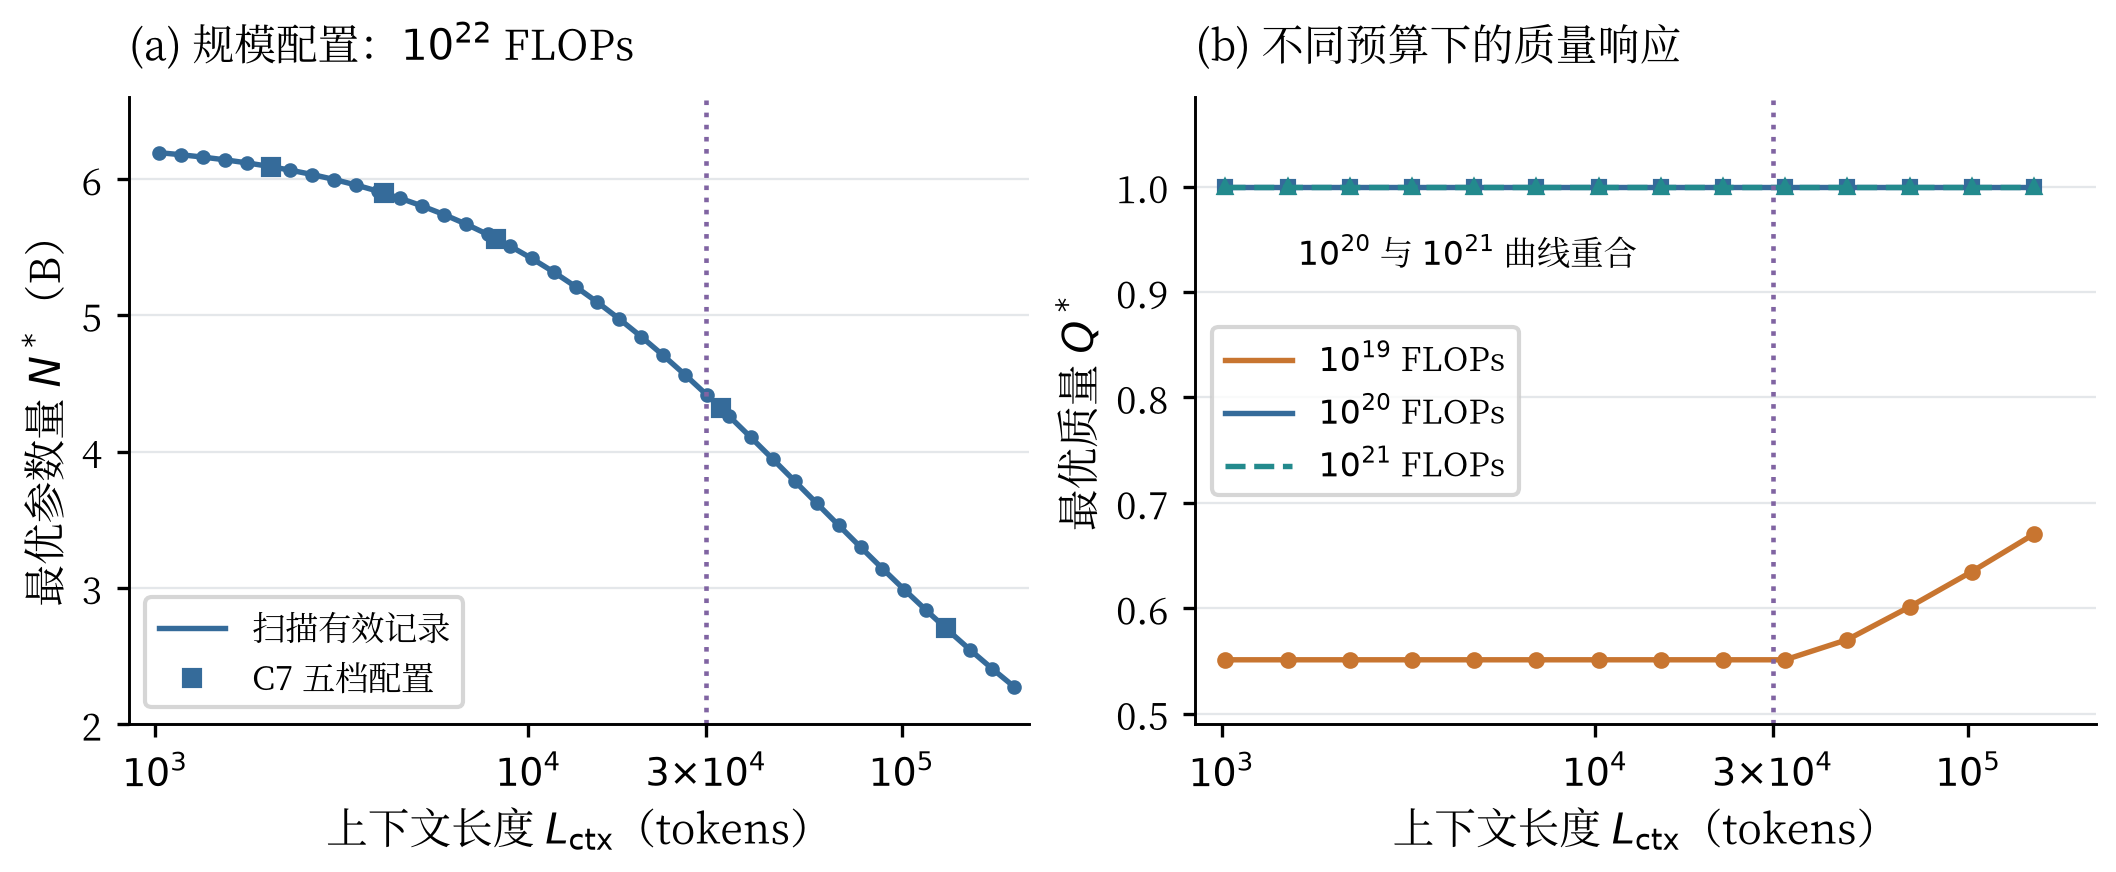
\includegraphics[width=0.94\textwidth]{../求解/问题三/图片/图3_上下文长度敏感性.png}
 \caption{上下文敏感性}
 \label{fig:p3_ctx}
\end{figure}

低预算的质量变化则不同。图\ref{fig:p3_ctx}右图中，$10^{19}$ FLOPs 的质量由 0.549 上升到约 0.671。按题设，质量处理总费用与数据量 $D$ 成正比；上下文延长后，可负担的数据变少，处理整份语料所需的费用也改变了，因此质量与规模之间的取舍随之变化。这一解释依赖当前的数据量成本关系。

\FloatBarrier

\textbf{4.固定配比平移的条件算例与适用范围}\par\nopagebreak[4]
领域配比会影响预训练效果\cite{xie2023doremi}。按问题一核岭预测的 $M=-0.1730$，保持共同费用基线，在 $10^{22}$ FLOPs 下得到相同的 $N,D,Q$，损失从 2.1451 平移至 1.9721。参考配比达到后一损失的模型等效预算约为 $1.691\times10^{23}$ FLOPs，即 16.9 倍。该换算依赖绝对损失差跨尺度不变，不能解释为实际训练加速比。

表\ref{tab:q23_review_m_amplitude}将收益幅度依次保留 $0$、$25\%$、$50\%$、$75\%$ 和 $100\%$，在满分配置下独立反解预算。全部幅度对应的 16.90739 倍与正式计算一致；仅保留一半时降至 3.49 倍。可见，等效预算对迁移幅度较敏感，这些人为设定的比例也没有置信区间含义。

\begin{table}[htbp]
 \centering
 \caption{固定损失平移幅度的条件算例}
 \label{tab:q23_review_m_amplitude}
 \renewcommand{\arraystretch}{1.15}
 \begin{tabularx}{0.94\textwidth}{@{}>{\raggedright\arraybackslash}X*{5}{>{\centering\arraybackslash}p{0.105\textwidth}}@{}}
 \toprule
 假定收益保留比例 & 0 & $25\%$ & $50\%$ & $75\%$ & $100\%$ \\
 \midrule
 等效预算倍数 & 1.00 & 1.81 & 3.49 & 7.30 & 16.91 \\
 \bottomrule
 \end{tabularx}
\end{table}

固定配比项只平移目标函数，成本或上下文变化则会移动预算边界，两类情景因此产生不同作用。另将核岭候选自身质量 0.5182 仅作为费用基线，在 $10^{22}$ FLOPs 下得到约 6.104B 参数、228.5B tokens，变化较小但不再完全相同。闭合参考质量 0.548753 对应的对照则约为 6.09049B、229.44095B。两项均另列保存，正式配置继续使用外生 $Q_0$。

质量未到上界时，新增预算同时影响质量和规模；达到上界后，质量处理继续付费，预算份额随模型扩大而降低。低预算尤其依赖处理成本，上下文则通过训练单价改变可用的数据量。把这些数值用于实际训练，还需核对评分尺度和外推范围，并确认高预算所需语料能否取得。数据受限训练研究已指出，重复使用数据的收益会递减\cite{muennighoff2023scaling}。本文尚未加入供给与重复训练约束，高预算解因此作为理论情景使用。

各情景共同采用问题二的点估计参数，结果表刻画的是这些参数给定时的配置差异。参数估计误差尚未转换为配置区间，因而表中精确到小数位的规模不应被理解为同等精度的工程需求。本文能够支持的是在既定评分、损失与费用关系下比较投入方向；实际资源安排还需结合可用语料、模型架构及任务要求判断这些条件是否成立。
\FloatBarrier
\endgroup
